\documentclass[fleqn]{report}
\usepackage{geometry}
\usepackage{amssymb}
\usepackage{fancyhdr}
\usepackage{multicol}
\usepackage{blindtext}
\usepackage{color}
\usepackage[fontsize=16pt]{fontsize}
\usepackage{lipsum}
\usepackage{pgfplots}
\usepackage{physics}
\usepackage{mathtools}
\usepackage[makeroom]{cancel}
\usepackage{ulem}

\graphicspath{ {../Images/} }
\setlength{\columnsep}{1cm}
\addtolength{\jot}{0.1cm}
\def\columnseprulecolor{\color{blue}}
\date{Spring 2025}

\newcommand{\textoverline}[1]{$\overline{\mbox{#1}}$}

\newcommand{\hp}{\hspace{1cm}}

\newcommand{\const}{\textrm{const}}

\newcommand{\del}{\partial}

\newcommand{\pdif}[2]{ \frac{\partial #1}{ \partial #2} }

\newcommand{\pderiv}[1]{ \frac{\partial}{ \partial #1} }

\newcommand{\comment}[1]{}

\newcommand{\equations} [1] {
\begin{gather*}
#1
\end{gather*}
}

\newcommand{\numequations} [1] {
\begin{gather}
#1
\end{gather}
}

\newcommand{\twovec}[2]{ 
\begin{pmatrix}
#1 \\ 
#2
\end{pmatrix}
}

\title{PHYS 498}
\author{Aiden Sirotkine}

\begin{document}

\pagestyle{fancy}
\maketitle
\tableofcontents
\clearpage

\chapter{PHYS498}
a whoooole lotta data analysis and fun stuff like that. 

\section{Clustering}
group together sample data points that are a certain distance from each other 
\[
d(i, k) = \sum\limits_{\textrm{features } i} (x_{ji} - x_{ki})^2
\]

However, what if data points have different units?

ML algorithms are "unit-agnostic", which means they don't really care about units. 

\section{Whitening Transformation}
\[
x \rightarrow \frac{x - \mu}{\sigma}
\]
it makes the mean 0 and the standard deviation 1

It just removes the white noise from a dataset. 

a whitening transformation is a linear transformation that 
transforms a vector of random variables with a known covariance matrix 
into a set of new varariables whose covariance is the identity matrix, 
meaning that they are uncorrelated and each have unit variance. 

whitening the inputs is useful because machine learning likes standardized data. 

\section{Examples}
you slam bags of apples together and columnated jets of walnuts come out 

\subsection{Atlas}
We look at the random jets of energy and we cluster the data to figure out 
what particles are where. 

\subsection{Gamma Ray Bursts}
We can look into the universe and see random bursts of gamma rays 

We find clusters of bursts at the galactic plane and around the center of 
the galaxy. 

We cluster the data and discover the Fermi Bubble. 

They're produced by colliding neutron stars and collapsing normal stars 
into black holes. 

\section{K-means Clustering}
fast and robust decent algorithm. Assume you data consists of roughly 
round clusters of roughly the same size. 
\[
\textrm{
a\_fit = cluster.KMeans(n\_clusters=2).fit(a\_data)
}
\]

\section{Hyperparameters}
parameters that have to be pre-set that determine how the data is going 
to be analyzed. 

For example, the number of clusters that we want as a result from K-means 

\section{ML Algorithms}
Maximize the goal functions given the data. 

The goal function $\mathcal L$ of the KMeans algorithm is 
\[
\mathcal L(c_j) = \sum^n_{i = 1} \sum_{c_j = i} |x_j = \mu_i|^2
\]
where $c_j = 1$ if the sample $j$ is assigned to cluster $I$ or otherwise 
$c_j = 0$ and 
\[
\mu_i = \sum_{c_j = i} x_j
\]

\subsection{Expectation-Maximization}
real important for alot of algorithms but I don't fully understand it. 

\section{Curse of Dimensionality}
$r^D$ is the volume of a D-dimensional hypercube with each dimension subdivided 
by $r$ partitions. 

a $3 \times 3$ rubix cube has 27 mini cubes in it because $3^3$

It basically means that the more dimension you have, the more cooked you are to process all of it. 

The curse of dimensionality. 

If we have 30 dimensional data, we need over 1 billion data points in order 
to get a sample in each partition. 

If there's a functional dependence between demensions, you can use a 
transformation to get rid of it and then you're working with less 
dimensions which is a win. 

In the slides, 500 dimensional data can get transformed into 2 dimensional data. 

\section{Linear Decompositions}
solve the eigenvector eigenvalue problem and delete the unimportant vectors and 
boom removed the most useless dimensions. 

Principle Component Analysis (PCA) was developed in 1901 and is 
basically just removing the smallest/least impactful eigvenvectors 

\subsection{Covariance Matrix}
\equations{
    C = \frac{1}{N - 1} X^T X
}
is an estimate of the true covariance matrix using the data $X$ 
comprised of $N$ samples that are $D$-dimensional. 

$M$ is matrix where each row is an eigenvector 

$Y$ is a matrix such that $X = Y M$

Remove dimensions from $D$ to $d$ with the smallest eigenvalues. 

Now you have a much smaller matrix with most of the same data. 

\subsection{Eigenmatrix of $X^T X$}
\equations{
    M^T = M^{-1}
    \hp 
    M M^T = I
    \\
    X^T X = M^T \Lambda M 
}
Where $\Lambda$ is the diagonal matrix of decreasing eigenvalues. 

The resulting latent variables are not correlated to each other, 
which means 
\equations{
    \rho(j, k) = \frac{Y_J \cdot Y_k}{|Y_j||Y_k|} \simeq 0
}

\section{Factor Analysis}
another good way to reduce data 

\subsection{Non-negative Matrix Factorization}
another thing 

\section{Independent Component Analysis}
another thing 

These aren't really important but like depending on what data you're 
doing you might need more than PCA. 

\section{Kernel Functions}
If you add a bunch of random ass dimensions to your data, you 
can observe a number of correlations that you would 
not have seen otherwise 
\equations{
    \phi(x_0, x_1)
    =
    \begin{bmatrix}
        x_0^2 \\
        x_0 x_1 \\
        x_1 x_0 \\
        x_1^2 \\
        \sqrt{2c} x_0 \\
        \sqrt{2c} x_1 \\
        c 
    \end{bmatrix}
}
This kernel function yields shenanigans 
\equations{
    \phi(X_i) \cdot \phi(X_j) = (X_i + X_j + c)^2
}
This allows you to embed your data into higher dimensional space 
without actually using a bunch of math. 

Our kernel function will be written as 
\equations{
    K(X_i, X_j) = 
    \phi(X_i) \cdot \phi(X_j)
}
A kernel function is a similarity measure, since it measures the 
similarity between samples $i$ and $j$, with identical values being 
maximal and orthogonal values being minimal. 

This is known as the kernel trick. 

Sadly there are not an infinite number of kernel functions $K$ 
\equations{
    K(X_i, X_j) = (\gamma X_i \cdot X_j + c)^d
}
is called the polynomial kernel.
There's also a sigmoid kernel and an infinite dimensional kernel 

\equations{
    K(X_{i}, X_{j}) = \exp(\gamma |X_i - X_j|^2)
}
Because of the taylor expansion of $e^x$, this kernel function 
yields an infinite dimensional expansion. 

\subsection{Kernel PCA}
goated method, but the data cannot be reconstructed super easily. 

It uses the kernel function to expand the data to a bajillion features, 
and it then uses PCA to take out only the best features.

However, you need your hyperparameters to not suck. 

\section{Local Linear Embedding}
Developed in the year 2000 which is more recent than most of the stuff we've 
done lol 

a type of \textit{Manifold Learning} (another way to reduce dimensions 
for non-linear data)

The sample is basically linear if you don't go too far away, so we 
can use a local linear approximation 
\equations{
    \vec X_i \simeq \sum_{j \neq i} W_{ij} X_j
}
and we find that matrix $W$ using a minimizing function 
\equations{
    \sum_i |\vec X_i - \sum_{j \neq i} W_{ij} X_j|^2
}
We've now found a set of weights that described the non-linear geometry 
of the sample data 

This geometry can be transferred to another sample space 
using another minimizing function 
\equations{
    \sum_i |\vec Y_i - \sum_{j \neq i} W_{ij} Y_j|^2
}

\chapter{Probability Theory and Density Estimation}
\section{Axioms of Probability}
\begin{enumerate}
    \item 
    A sample space $\Omega$ that defines the set 
    of all possible uncertain outcomes 
    \item 
    An event space $\mathcal F$ of combinations 
    of outcomes (subsets of $\Omega$)
    \item 
    A probability measure $P: \mathcal F \to [0, 1]$
    that assigns numerical probabilities to each event. 
\end{enumerate}

The tuple $(\Omega, \mathcal F, P)$ is a probability space 

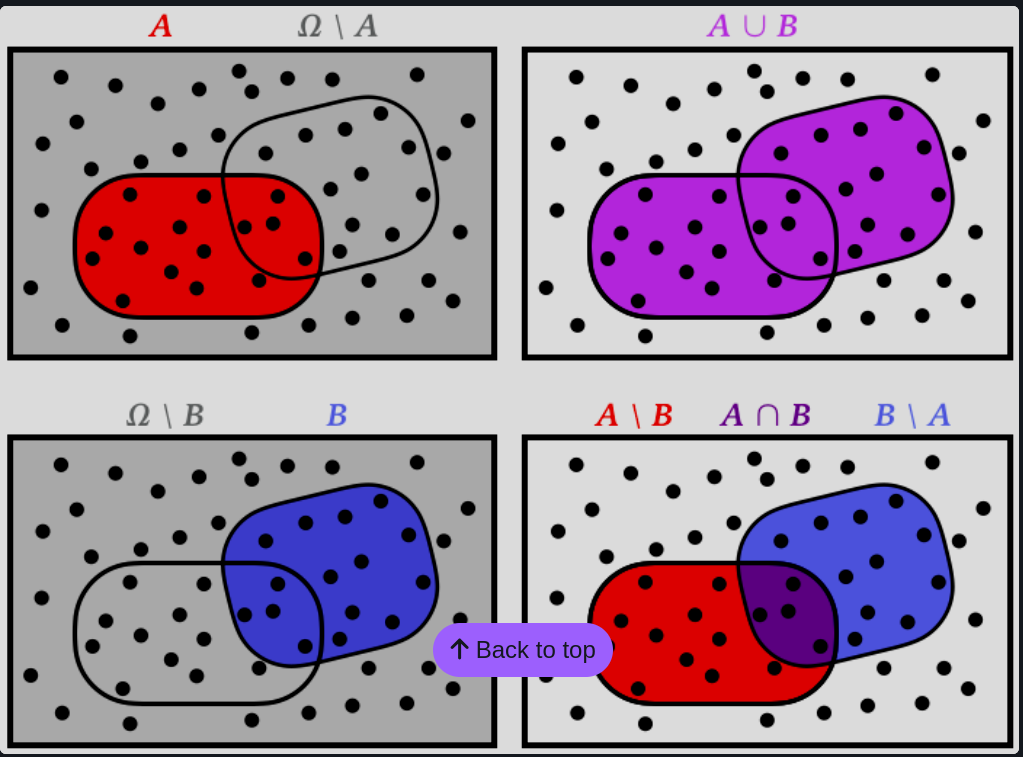
\includegraphics[width = 14cm, height = 10cm]{PHYS498.1.png}

An event space must satisfy the following conditions
\begin{itemize}
    \item 
    If event $A$ is in the event space, then so is its complement $\Omega / A$
    \item 
    If events $A_1$ and $A_2$ are included, then so is their union $A_1 \cup A_0$
\end{itemize}

\subsection{Kolmogorov Axioms}
\begin{itemize}
    \item 
    For any event $A$, $P(A) \geq 0$ 
    \item 
    $P(\Omega) = 1$
    \item 
    if all events have no outcomes in common, then 
    \[
    P(A_1 \cup A_2 \ldots ) = P(A_1) + P(A_2) \ldots
    \]
\end{itemize}

\subsection{Bayes' Rule}
The probability of $A$ given $B$ 
\[
P(A | B) \equiv \frac{P(A \cap B)}{P(B)}
\]

If $A$ and $B$ are independent, then 

\[ 
P(A | B) = P(A) 
\]

and then 
\equations{
    P(B | A) = P(A | B) \frac{P(A)}{P(B)}
}

Bayes' Theorem comes in handy for the disease test false positive shenanigans. 

\section{Random Variables}
Let a random variable $X: \Omega \to \mathrm{R}$ labels 
each possible outcome $\omega \in \Omega$ with a real number $x = X(\omega)$

The probability is defined to be 
\equations{
    P(X = x) \equiv P(\{ \omega: X(\omega) = \omega \})
}

\section{Cumulative Distribution Function}
\equations{
    F_X(x)
    \equiv 
    P(\{
    \omega: X(\omega) \leq x    
    \})
}
It rises monotonically from $0$ to $1$ and is always well defined

\section{Probability Density Function}
\equations{
    f_X(x) \equiv 
    \frac{d}{dx} F_X(x)
}

A PDF is a density function in the sense that 
\equations{
    P(\{ \omega x \leq X \leq x + \Delta x \}) 
    \simeq 
    f_X(x) \Delta x
}

\subsection{Kernel Density Function}
It's something 

\subsection{Gaussian Mixture Model}
It's another algorithm that's good at grouping and density estimation. 

\section{Monte Carlo Method}
Instead of integrating over a range, you can just take a random 
sampling to find the average over a function 
\equations{
    \langle g \rangle 
    \equiv 
    \iint 
    dx \, dy \, 
    g(x, y) P(x, y)
}
We can use the standard deviations of $x$ and $y$ to find 
the correlation between the two 
\equations{
    \sigma_x^2 = \langle (x - \overline{x})^2 \rangle 
    \\
    Corr_{xy} = \langle ((x - \overline{x})(y - \overline{y})) \rangle 
}
You can use that to find the correlation coefficient 
\equations{
    \rho 
    \equiv 
    \frac{Corr_{xy}}{\sigma_x \sigma_y}
}

\subsection{Covariance Matrices}
Useful 

\chapter{Probability}

\section{Jensen's Inequality}
Convex functions are nice because you can find the global maximum very easily. 
\[
g(\langle \vec x \ldots \rangle )
\leq 
\langle g(\vec x) \rangle 
\]
The function at the expected value is always less than or equal 
to the actual expectation value of the function. 

\section{Probability Interpretations}
\subsection{Frequentist}
Frequentist statistics means that the probability of an event 
is determined by the law of large numbers (the ratio of successes 
 and failures will reach the probability with enough trials)

This is flawed for non-repeatable experiments (2016 NBA Finals)

\section{Bayesian}
You just like believe something has a certain chance based on past data. 

Consider a joint probability distribution 
\equations{
    P(D, \Theta_M, M)
}
with data features $D$, paramethers $\Theta_M$, and 
hyperparameters $M$.

If we consider like the spins of subatomic particles, we 
have to consider the possibility that an event occurs even if 
it has never occured before. 

\subsection{Likelihood}
Returns the probability density of observing $x$ given 
parameters and hyperparameters 
\equations{
    \mathcal L_M(\Theta_M, \vec x)
    =
    \sum^K_{k = 1}
    \omega_k G(\vec x; \mu_k, C_k)
}
with parameters $\omega, \mu, C$.

\subsection{Bayesian Inference}
\equations{
    P(\Theta_M | D, M)
    =
    \frac{P(D | \Theta_M, M) P(\Theta_M | M)}
    {P( D | M)}
}
posterior = likelihood * prior / evidence

prior knowledge and new information $\rightarrow$ new knowledge. 

\subsection{Dice}
Supposed you are given 3 dice rolls and have to guess how 
many sides are on the rolled dice.

The options are d4, d6, d8, d12, d20. 

The dice rolls 6, 5, 4

It's definitely not a 4 sided die 

If we guess the rolls are close to the mean, then its probably not 20 sided. 

You can do some math and show that the most likely dice that was rolled was 
a d6. 

\subsection{Prior Probability}
If your posterior data is greatly affected by your prior data, then you need more 
prior data. 

A decent experiment's worth of data should be strong regardless of prior data. 

You can also use an integral to compute Baye's rule over a range 
\[
P(D | M)
=
\int d \Theta_M' P(D | \Theta_M' , M)  P(\Theta_M' | M)
\]

\section{Graphical Models}
graph CS not graph cartesian 

Big probabilities can be turned into smaller joint probabilities. 
\equations{
    P(D, \alpha, \beta)
    =
P(D, \beta | \alpha ) P(\alpha )
=
    P(D | \alpha, \beta)
    P( \beta | \alpha)
    P(\alpha)
}

There's some pictures on the website 

\chapter{Markov Chain Monte Carlo}
Generate random samples from a non-normalized probability density 
\equations{
P(\vec z) = 
\frac{f(\vec z)}{\int d \vec z \, f(\vec z)}
}

You can find a half decent sampling using importance sampling 
\equations{
    \langle g(\vec z) \rangle 
    \equiv 
    \int d \vec z \, 
    g(\vec z) P(\vec z)
    =
    \frac{1}{N}
    \sum^N_{i = 1}
    g(\vec z_i)
}

A random sampling of the MCMC data yields roughly the normalized integral 
\equations{
    \frac{f(z)}{P(z)} = \int dz \, f(z)
}

\section{Stochastic Processes and Markov-Chain Theory}
Generates a sequence depending on all past data points in the sequence.

These processes end up making random distributions. 

\subsection{Markov Chain}
It's a probability graph where the $n$th sample depends only on the $(n-1)$th 
sample. 

It's a stochastic process with an extremely short term memory.

After enough time, the correlation between a stochastic process 
and its initial conditions decreases.

We talked about these guys in lin-alg they're pretty cool.

\subsection{Stationary}
The update rule is always the same 

The probability of the M2 given M1 is the same as M3 given M2 

so you can iterate forever 

Markov chains reach an equilibrium after a while based on some eigenvectors. 

After a bajillion iterations for stationary markov chains, the 
dependence on the initial values entirely disappears. 

Works for all stationary markov chains.

You get a probability density 

Markov chains are reversible if there symmetry along the diagonal axis $y=x$

\subsection{Custom Markov Chains}
Metropolis-Hastings-Green algorithm is an algorithm for making a 
markov chain with a pre-determined probability density.

\subsection{Markov-Hastings}
It relies on a proposal distribution that is easier to 
sample from than the target distribution.

You can choose any proposal distribution, but you should choose one 
that is similar to your actual probability density to get to equilibrium 
faster. 

There's a formula in the lecture notes. 

\subsection{Gibbs Sampling}
another type of MH algorithm 

If we want to sample a 3d distribution, we take 3 different samples of 
the conditional probabilities. 

You end up getting something that is proportional to the true 3d sample 

\subsection{Hamiltonian Sampling}
Calculate all partial derivatives of our target $\log(\tilde{P})$

You do some Hamiltonian witchcraft that I probably would maybe understand 
if I took 325 and then you get a distribution. 

Canonical Distribution. 

\section{Bayesian Model Selection}
We remember Baye's Rule, but now we have to figure out what model 
we should use to get the best probabilities. 

\equations{
    P(\Theta_M | D, M)
    =
    \frac{ P(D | \Theta_M, M) P(\Theta_M | M) } { P(D | M) } 
}
We need to figure out a model M to use 

We have a number of methods that we can use that are all in the slides. 

If we do pairwise comparision, then the probabilty of the evidence 
cancels out and we don't have to deal with it. 

\equations{
    \textrm{Baye's Factor }
    =
    \frac{P(D | M_1)}
    {P(D | M_2)}
}

Bayesian inference is a fan of Occam's Razor: the simplest model 
without prior evidence is the most likely model. 

We can imagine the same thing with 1 big gaussian or 2 small guassians 
being the differing models for a certain data set.

There's a Jeffrey's Scale that's basically just metric 

100 is very strong M1, 10 is kinda likely M1, 0.1 is kinda likely M2, 
0.01 is very strong M2. 

Model is real involved you should come back to this. 

\section{Variational Inference}
VI provides an exact description of an approximate posterior distribution 
(using optimization).

MCMC provides an approximate description of the exact posterior 
probability density using sampling.

\subsection{Kullback-Leibler Divergence}
It's a formula to determine how "close" two functions are to each other. 
\equations{
    KL(q || p) 
    =
    \int 
    q 
    \log(
    \frac{q}{p})
}

It can also be considered the difference in the expected values 
between the logs of $q$ and $p$

There's then more stuff 
\equations{
    P(\theta) = 
    P(\theta | D )
    =
    \frac{P(D | \theta) P(\theta)}{P(D)}
    \\
    KL(q || p)
    =
    \ln(P(D))
    +
    KL(q || P)
    -
    \int d \theta q(\theta) \ln(P(D | \theta))
}
and those last 2 terms are called ELBO for some reason. 

$
    KL(q || P)
    -
    \int d \theta q(\theta) \ln(P(D | \theta))
$
is the evidence lower bound (elbo)

\subsection{Variational Inference Method}
Take a sample function and minimize the KL divergence to find the sample 
function that most closely approximates our probability density.

You can calculate the KL divergence and find the minimums 
of certain functions analytically. 


\section{Evidence Lower Bound}
remember Baye's rule 

\equations{
    p(\theta) = 
    \frac{P(D | \theta) p(\theta)}{P(D)}
}
The probability of the model is the probability of the data given the model 
times the probability of the data divided by the evidence. 

\subsection{Variational Bayesian Inference}
define a family of functions that could approximate the posterior 
probability density. 

Use optimization to find the best function 

\equations{
    P(\theta) = 
    P(\theta | D )
    =
    \frac{P(D | \theta) P(\theta)}{P(D)}
    \\
    \int \, d\theta \, 
    q(\theta)
    \left(
        \ln(P(D))
        +
        \ln(\frac{q(\theta)}{P(\theta)})
        -
        \ln(P(D | \theta))
    \right)
    \\
    KL(q || p) 
    =
    \ln(P(D))
    +
    KL(q || P)
    -
    \int d \theta q(\theta) \ln(P(D | \theta))
}
and those last 2 terms are called ELBO for some reason. 

$
    KL(q || P)
    -
    \int d \theta q(\theta) \ln(P(D | \theta))
$
is the evidence lower bound (elbo)

\begin{itemize}
\item
The three terms are the log of the evidence $P(D)$, 
\item
THe KL divergence of $q(\theta)$ with respect to the prior 
\item
and the q-weighted log-likelihood of the data
\end{itemize}

The log of the evidence is a constant offset in the sum 

the KL divergence is minimized when $q(\theta) = P(\theta)$

the log-likelihood is minimized when $q$ prefers 
parameters that explain the data 

\equations{
    \ln(P(D))
    =
    \int d \theta q(\theta) \ln(P(D | \theta))
    -
    KL(q || P) 
    -
    KL(q || p)
    \\
    \ln(P(D))
    \geq 
    \int d \theta q(\theta) \ln(P(D | \theta))
    -
    KL(q || P) 
    \\
    ELBO
    \equiv  
    \int d \theta q(\theta) \ln(P(D | \theta))
    -
    KL(q || P) 
}

Using this, we also find that 
\equations{
    KL(q || p) 
    =
    \ln(P(D))
    -
    ELBO(q)
}

The evidence based lower bound can be written as the sum 
of a bunch of expectation values 
\equations{
    ELBO(q)
    =
    \langle 
        \ln(P(D | \theta))
    \rangle_q 
    +
    \langle 
        \ln(P(\theta))
    \rangle_q
    +
    \langle 
        \ln(q)
    \rangle 
}

\subsection{Example (Laplacian PDF)}
the probability of observing $x$ given some model parameter $\theta$ is 
\equations{
    P(x | \theta)
    = 
    \frac{1}{2}
    e^{-|x - \theta|}
}

So our resuling likelihood is 
\equations{
    P(D | \theta)
    =
    \prod_i P(x_i | \theta)
}

Let our prior knowledge be specified by a unit Gaussian (approximate 
function)

so our posterior probability density function is 
\equations{
    P(\theta | D)
    =
    \frac{P(D | \theta)P(\theta)}{P(D)}
}

Now we let our approximate function be a unit Gaussian to optimize. 

\subsection{Practical Applications}
Markov Chain Monte Carlo always gives you something 
as long as you have a likelihood and prior. 

VI is generally more computationally efficient, but takes a little more 
to set up. 

It takes some amount of judgment and prior knowledge to have a decent 
approximating function $q$

\section{Optimization}
real important math 

\equations{
    x^* = \textrm{argmin} f(x)
}

The easiest way to approximate the minimum is just sample 
over the entire function and take the smallest result, but this 
is not very accurate. If you sample distances are too big, you'll miss details 

\subsection{Gradient Descent}
make constant small steps in the direction perpendicular to the gradient 

$\eta$ is the learning rate and determines how big of jumps you make per step. 

You can find the gradient by calculating 
derivatives numerically 
\equations{
    \frac{\del}{\del x_i} f(x)
    =
    \frac{f(x + \delta e_i) - f(x - \delta e_i)}{2 \delta} + \mathcal O(\delta^2)
}

Very fast, but not super accurate 

\subsection{Auto-differentiation}
a hybrid between the difference equations and an analytical approach 

You take a number of primitive functions and you numerical 
factors to optimize those primitives to your real function. 

It's extremely fast and extremely accurate. 

Doesn't work for diverging points 

If you just put a value there then everything works. 

\subsection{Optimization in Machine Learning}
K-means clustering is just an optimization function that optimizes 
\equations{
    \sum^{n}_{i = 1}
    \sum_{c_j = 1}
    |x_j - \mu_i|^2
}

Optimization is also useful in Bayesian Inference. 

consider the maximum a-posteriori (MAP) point estimate 
\equations{
    MAP 
    \equiv 
    \textrm{argmin}_{\theta} ( - \ln(P(\theta | D)))
}

You can see the MCMC calcualtion with the MAP estimate 

You can also find the maximum likelihood (ML) point 
\equations{
    ML 
    \equiv 
    \textrm{argmin}_\theta (-\ln(P(D | \theta )))
}

You also see optimization is Variational Inference 
\equations{
    VI
    \equiv 
    \textrm{argmin}_{\lambda}
    (
        -ELBO(q(\theta; \lambda) || P(\theta | D))
    )
}

\subsection{Optimization Methods}
There are a bunch but just use the best one which is 
stochastic gradient descent. 

People benchmark their optimization functions based off of 
the Rosenbrock function. 

You use automatic-differentiation to get the gradient and then 
you use gradient descent to optimize the function and boom 

\subsection{Stochastic Gradient Descent}
gradient descent but use only a small sample subset of the function, 
called a minibatch. 

It takes more steps, but drastically reduces the amount of data necessary. 

the noise caused by SGD helps prevent overtraining by 
adding noise to the data. 

\section{Cross Validation}
There are 3 types of learning 
\begin{itemize}
    \item 
    learning model parameters from data 
    \item 
    Learning to predict new data (unsupervised learning)
    \item 
    Learning to predict target features in new data (supervised learning)
\end{itemize}

All three of these models require previous data to do anything. 

Now we have to figure out how to compare models to learn which is best. 

Bayesian evidence is the main tool to see which model is preferred by 
the data. 

The way you do this is with multiple different datasets
 
\subsection{Training Set}
This is how you initially train the model you make your initial curve 
fitting parameters. 

\subsection{Validation Dataset}
After the model has been trained, you evaluate the model based on new data, 
but you still tune the model's hyperparameters while it looks at the validation set. 

Mainly for fine tuning. Hopefully you don't need to make major changes 
after the model has gone through the training data. 

YOU CAN ONLY CHANGE THE HYPERPARAMETERS, YOU CAN'T CHANGE THE MAIN PARAMETERS.

\subsection{Test Dataset}
Once the algorithm is completely trained, you give it unseen data as a final 
test to see if your model is any good in a real world scenario. 

\section{Cross Validation Process}
We will study the \textit{K-folds} method of cross validation. 

\subsection{Overfitting and Generalization}
Competing models can be considered as $P$ order polynomials with $P+1$ parameters.

You can use linear regression to implement a fit and 
then make a pipeline (python library)

An overfit model will go over too many data points but not get the big picture. 

An underfit model does not have enough parameters so it is also missing the 
big picture. 

\subsection{Train-Test Split}
There's a python library that automatically cross-validates data. 

Somewhere between 10\% and 50\% (sklearn automatically does 20)
is a decent split for training data and testing data. 

\section{K-Folding}
Split the data multiple times and combine the correlated results. 

The more k-fold splits you make, the more correlated your data will be. 

It's called K-Folding because you split the data to roughly $k$ samples 
of roughly $k$ datapoints. 

It works pretty well but you have to check your polynomial degrees to 
prevent overfitting 

\section{Comparison with Bayesian Evidence}
We can use MCMC to calculate Bayesian evidence. 

\chapter{Artificial Intelligence}
\section{Intro}
skip 

\section{Supervised Learning}
Instead of doing Bayesian evidence probability stuff, supervised learning 
is trying to map data to results and eventually get a function that 
acts as a predictor (hypothesis).

A regression problem maps stuff to stuff continuously. 

A classification problem maps all stuff to some discrete number of things. 

\subsection{Linear Regression}
Matrix math to make a best-fit line. 

There's some probability stuff and some error math but I missed it 

\subsection{Linear Deconvolution}
We are trying to find the response function of the system. 

The response function is function such that 
\equations{
    z'(t) = 
    \int \, dt' \,
    R(t - t') z_{input}(t')
}
This is called a convolution. 

So we're going to use a linear model to try and deconvolute 
the convolution. 

The issue is when there's any noise in your model, the deconvolution 
becomes horrendous.

Deconvolution amplifies noise. 

\subsection{Regularization}
Use fancy math to minimize the noise in a model so that 
deconvolution actually works well. 

\chapter{Artificial Intelligence}
AI is a computer doing human-level reasoning 

ML is a computer learning without explicitly being programmed. 

Artificial Neural Networks have node and hidden layers and whatnot 

Deep Learning is an ANN with more than 3 layers. 

You have a number of different types of learning 
\begin{itemize}
    \item 
    Supervised 
    \item 
    Unsupervised 
    \item 
    Semi-supervised 
    \item 
    Reinforcement
\end{itemize}

Supervised Learning is defined by how data is labeled.

Unsupervised learning just recognizes patterns

Deep Reinforcement learning is very very time consuming and requires a 
whole lot of data. 

inputs go into a black box that makes outputs. 

\section{Neural Network}
Generic, flexible, trainable, modular, and efficient.

It's pretty good and can map most non-linear functions. 

Given some data, you mulitply it by a weight and then 
plug it into some activation function.

\subsection{Network Layer}
Consider the weight as a matrix instead of just a constant. 

There are all sorts of different decision boundaries depending on your 
activation function.

We take a tensor of input data and it goes through a number of weighted matrix 
multiplications until we get some output tensor. 

\subsection{Tuning}
You can look at the results of the function.

If we calculate the mean squared error and set its derivative to 0 
then we can do some math to tune our ML model.

\section{Pytorch}
It allows you to make an ML model pretty easily. 

It randomly makes the weights.

\section{Loss Functions}
This is really the thing that Gradient Descent is talking about 
\equations{
    \theta \rightarrow 
    \theta_i - \eta \frac{\del l}{\del \theta}
}
Wherer $l$ is your loss function. 

You find a loss function and then you calculate the gradient 
and then good things happen. 

\subsection{Regression Loss}
This is the way that regression functions in lin alg work. 
It's basically just the squared error 
\equations{
    L_2 
    =   
    \frac{1}{2}
    |X_{out} - Y_{tgt}|^2
}

Minimizing the loss is the same as finding the maximum likelihood 
point estimate 

\subsection{Binary Classification Loss}
The binary cross entropy is a better loss function for binary 
classification problems (cat or dog (or whatever))

The equation is in the thingy

most code uses either BCE or MSE loss.

What is MSE loss though?

\subsection{Multicategory Classification Loss}
This is another crazy loss function that uses some math 
to optimize for if there are multiple discrete categories that you 
are trying to match. 

This is all related to Bayesian Variational Inference (VI)

The K-L Divergence when grouping stuff like a month ago 
is also related to the minimizing loss functions. 

\subsection{Deep Neural Networks}
MLP - Multi-Layer Percepteron 

You connect layers of nodes to new layers of nodes until something 
good happens.

You can drop out random neurons to test how robust the neural network out. 

You can have nodes feed back into themselves (Recurrent NN)

You can have Auto Encoders and Variational Auto Encoders.

A GAN is a Generative Adversarial Network.

Neural Networks can approximate universal functions. 

Deep learning just needs data instead of outside feature extraction. 

\subsection{Minibatch Gradient Descent}
You batch your gradient descent steps and as long as your batches are 
small enough you reduce compute time without reducing error. 

\section{Generalization}
Avoid underfitting and overfitting 

In underfitting, your validation and training error are about the same 

In overfitting, you training data has very low error but your validation 
error is too high. 

\subsection{Drop Out}
A good way to generalize your function is Drop Out 

Just get rid of 20-50 \% of your nodes 

\subsection{Early Stopping}
watch how your validation error changes and stop when the validation 
error goes up. 

\section{Convolutional NNs}
Mainly used for image data. 

They use a convolutional operator to extract data features. 

These NN's are robust against spatial translation (they 
can find the same features even if theyre in different parts of the image)

It takes larger image and turns it into less data using the convolutional 
function. 

You can have multiple layers of convoluting and max pooling to turn a 
whole bunch of data into a little bit of feature data. 

Far better for image processing than regular feed-foward networks because 
the convolution compresses the data. 

\subsection{Caveats}
Data has to be put on a regular grid. 

\section{Recurrent NNs}
Used for modelling sequential data (Language Models). Youre data is 
coming in a sequence.

It triggers recurring connections between neurons. 

RNN's can be used for basically anything as long as there is ordered data. 

Feed Forward NN's always move data from left to right. 

Recurrent NN's also allow for data to be left inside the network as new data 
is being inputted, allowing for some time of stochastic shenanigans (LLM's)

Because recurrent NN's use looping, they use far less nodes than deep NN's 
and can be put on something like an FPGA.

\subsection{Caveats}
The order of the data now matters. 

Input data needs to be packaged into variable-length messages 

Gradient Descent is possible but involves "unrolling" the nodes. 



\section{Long-Short Term Memory Networks}
You have an input gate, output gate, and a forget gate. 

It limits the amount of information that can be passed from one 
cell to the next. 

\section{NN talks}
We've had NN's for a while but they weren't useful until we thought about 
using non-linear activations functions (tanh, sigmoid)

We also use backpropogation to increase the strength of NN's

Skipping connections also made AI pretty good by increasing 
generaliztion. 

\chapter{Deep Learning}
It's real useful 

\section{Geometric Deep Learning}
Non-Euclidean data can represent more complex informaition. 

A non-euclidean datatype is a graph 

molecules are realy good examples of information that should be represented 
with a graph.

Nodes in a graph can have features. 

Tons of stuff can be represented in a graph (molecules, information, neurons, 
genes, communication networks, software)

\section{Graph Setup}
$V$ is the vertex set 

$A$ is the adjecency matrix (assume binary) 

$X \in \mathbb{R}^{|V| \times m}$ is a matrix of node features 

$v$ is a node in $V$, and has $N(v)$, which is the set of neighbors of $v$

\section{Naive Approach}
You just plug the adjacency matrix directly into the thingy.

There are $O(|V|)$ parameters.

It is not applicable to graphs of different sizes 

It is sensitive to node ordering.

\section{NN Invariants}
Deep NN's can "learn" translation, scale, rotations given enough data through 
the changes and shared features.

\section{Graph Neural Network}
A GNN is a class of GDL methods for modeling data via message passing 
over graphs 

GNN architectures ar edesigned to learn a nembedding that 
contains informaition about its neighborhood.

Relationships of increasingly distant nodes/edges incorporated iteratively 
through use of additional message passing steps. 

GNNs learn contextual relationships between nodes 

\subsection{LHC Example}
You have sensor at various distances, and you create a sparse graph 
of potential paths that the particles could have taken from where the sensors 
sensed a hit. 

The GNN returns true or false on given edges, and the true edges are the 
most likely paths that particles took. 

Once you train a GNN, you're able to determine the likely paths of particles 
extremely quickly without a ton of computer power. 

We have a bunch of nice python code in the website to 
show how GNN's work. 

\subsection{Graph Convolutional Network}
They're like GNN's except they also use a convolution function to reduce 
a full graph into important traits. 

\subsection{Deep Sets}
It's a deep neural network library that receives samples of a discrete 
set of data. 

There's a whole paper made in 2017 that talks about how it works.

\section{Attention}
From a paper called "Attention is All You Need". 

It talks about transformer models and how attention is used to improve 
deep learning models. 

Recurrent neural networks take in remembered data from previous samples. 

You can make a bidirectional RNN that determines information at time $t$ by 
looking at information both before and after $t$. 

Causal RNN's only predict future data given past data. 

The biggest issue with these RNN's is you eventually run out of memory. 

\subsection{Attention Augmented RNN}
It essentially gets the weight average of the correlations between tokens 
to figure out what parts of a sequence matter the most. 

This is related to convolutions because a convolution function summarizes a spread 
of data, and the attention function summarizes the past and present information. 

We use the softmax algorithm to weight our external data. 

You have QUERY, KEY, VALUE items and you have to find the similarities between 
QUERY and KEY. 

You do some matrix math and good things happen. 

Vectors that are closer together have larger dot projucts- more similar 
vectors yield a greater attention. 

Everything is matrix multiplication. 

\subsection{Enforcing Causality}
You can force certain parts of the attention matrix to be 0 depending on 
how our sample data is correlated to itself.

\subsection{No Learnable Parameters}
You can literally just compute the autocorrelation $X X^T$ 

\subsection{Crazy Amounts of Technicalities}
Just read the website lecture notes. 

\subsection{Cross Attention}
We have two different streams of data that relate to each other, and you 
need attention between streams of data. 

\subsection{Flash Attention}
It's something to do with GPU programming 

\chapter{Transformers}
Transformers are the thing that revolutionized the world like 3 years ago. 

They are very impactful in NLP (Natural Language Processing), but we won't go 
over that in crazy detail at the moment. 

Transformers are AI architecture that uses attention to predict data. 

Transformers are also very good at computer vision. 

\section{Attention DFN}
The attention mechanism describes a weighted averag eof (sequence) elements with the weights 
weights dynamically computed based on an input query and elements' keys. 

What transformers use mainly is self-attention. 

\subsection{Scaled Dot Product Attention}
We want an attention mechanism where any element can affect any other element, but 
the mechanism is still efficient to compute. 

You do some math and take the softmax of it. 

\subsection{Tilde}
A tilde ~ means to sample from a certain things 

$q_i ~ N(0, \sigma^2)$ means that $q_i$ is sampled from a normal 
distributed centered around 0 with a standard deviation $\sigma^2$

\section{Multi vs Single Headed Attention}
Multi-Headed attention essentially means you get multiple matrices that each 
can affect the data according to the attention. 

This allows you to look at multiple possible relationships between data. 

\section{Transformer Architecture}
It's on the website, but the main thing that its just a lot of multi-headed 
attention blocks in a feed forward network. 

Transformers utilize skip connections. 

\section{Positional Encoding}
We let the multi-headed attention network understand the relative positions of 
its data encoding it via an input feature.

We do some math to let the computer know the ordering of things.

We are trying to break the equivariance of the multi-headed attention. 

\section{Learning Rate Warmup}
We have to start the learning rate close to 0 and gradually bring the learning 
rate up to where we want it originally, and then it can go back down. 

\section{Multi-Headed Attention}
I only added this to really cement it as the important part of transformers.

Transformers are special because they have multi-headed attention compared 
to other attention-augmented neural networks.

The weighting based on dot product similarity and 

the batching of attention in transformers 

The weighting is also important 

\chapter{Generative AI}
Machine learning is a part of Artificial Intelligence, and 
Generative Models are a part of Machine Learning, and Deep Generative Models 
are a part of Generative Models and Deep Learning. 

\section{Discriminative vs Generative Models}
A discriminative model will, given a set of input data, distinguish (discriminate)
that data between various traits. 

Generative models can, given traits, make data that the discriminative AI 
will recognize as having that trait. 

Discriminative models learn a probability distribution given data $p(y | x)$ 

Generative models learn a probability distribution itself $p(x)$

Generative models can learn features without labels. 

Conditional Generative models can assign 
labels while rejecting outliers. It generates new data conditional 
on input labels. 

The way that generative models work is by converting noise to real data. 

\section{Types of Generative Models}
\begin{itemize}
    \item 
    GAN : Adversarial Training with a Discriminator 
    \item 
    VAE : Maximize variational lower bound with an Encoder 
    \item 
    flow based models : invertible transform of distributions 
    \item 
    Diffusion : Gradually add Gaussian noise and then reverse the noise 
\end{itemize}

The flow models uses invertible transforms and Jacobians. 

\section{Applications}
Generative models are generally not better than full simulations of data, but 
they are much cheaper and much faster, which is their real benefit. 

\section{Auto-encoders}
It turns data into less data while keeping the same information.

Specifically its a neural network that compresses data. 

\subsection{Mp4 Compresion}
`It takes reference images, and instead of storing every single pixel, it will 
just store the change in pixels between each image. Now our filesize is 
very small, but our CPU needs to do more work to turn the compressed 
data into the actual video. 

Autoencoders turn a bunch of redundant information into only the necessary 
information, with the rest being able to be extrapolated from an algorithm. 

Autoencoders do unsupervised dimensionality reduction.

\section{Curse of Dimensionality}
We need Autoencoders because without them, data becomes extremely expensive to 
do statistics on and impossible to interpret. 

\subsection{PCA}
It works great, but has some limitations 

Auto-encoders are non-linear PCA, and the components DO NOT have to be 
orthogonal to each other. 

\section{Training}
What your loss function is is the loss of information from encoding to decoding. 

You want to decrease the amount of space in your data whilst losing as little 
information as possible after decoding the reduced data. 

The way that you actually decrease the amount of data is by making a bottleneck
(smaller and smaller layers) such that less information can go through each 
layer. 

\section{Convolutional Autoencoder}
Instead of using regular matrix layers, you can put convolutional layers 
in an autoencoder to get dimensionality reduction. 

\section{Generation}
You can use the decoding part of an autoencoder as a generative AI. 

The issue with this is that the generational space is extremely large 
and not regularized, so sampling from it can yield absurd results. 

\section{Variational Autoencoder}
\begin{itemize}
    \item 
    You marry the Variational Inference method with autoencoders to reguarize 
    your inference space. 
    \item
    You use the KL Divergence relative to a unit Gaussian. 
    Basically we minimize the difference between our distribution and 
    a standard Gaussian. 
    \item
    What you do is you add an additional term to the loss function. 
    The additional term requires that the latent space variables are unit Gaussians. 
    \item
    Now our latent space is a multidimensional unit Gaussian. 
    \item
    Our big unit Gaussian latent space is essentially our noise that we can 
    sample from randomly to make image generation. 
\end{itemize}

\subsection{Generating Data}
It works pretty well, you just sample noise from out big thing of 
Gaussians and decode it to get an answer. 

The issue with variational autoencoders is that there is now a smooth 
transition between each sample, so the autoencoder will create a mix 
of every distinguishing trait instead of one at random. 

You need to add some sort of discretization in order to make specific traits 
from a variational autoencoder. 

\chapter{Generative Adversarial Networks}
These are called GAN's 

\begin{itemize}
    \item
    The way that they work is in tandem with a discriminatory neural network. 
    \item
    It essentially generates data until the discriminator NN says that the generated 
    data has the desired trait. 
    \item
    The discriminator is trained on real data, and tells the generative NN whether 
    or not the generated data has the corrected traits.
\end{itemize}

\section{Issues}
The main thing with GAN's is they are are very finnicky, and they can yield 
very large losses if not trained correctly. 

\subsection{Mode Collapse}
Sometimes a GAN will only generate 1 type of output or a small subset of outputs. 

If the discriminator gets stuck in a local minimum, then the generator can 
repeat the same output and not get trained successfully. 

\subsection{Vanishing Gradients}
When the discriminator is only slightly better than the generator, the update 
weights will disappear and it will stop improving. 

\subsection{Convergence}
The GAN's effectiveness will oscillate because the discriminator is so bad 
that it is essentially a coin flip. 

\section{Conditional GAN}
It allows the user to not only generate images, but to also label them with 
specific traits. 

\chapter{Diffusion}
% You take an image, transform it into noise, and then just take the inverse. 

\begin{itemize}
    \item
    You make a de-noising machine, and then you give it all noise and it 
    tries to generate an output. 
    \item
    Adding noise is easy, removing noise is hard 
    \item
    The noise is not specifically random, but is developed from a noise scheduler. 
    \item 
    The noise is always Gaussian. 
\end{itemize}

\section{Implementation}
You actually use Variational Inference to make the de-noiser because the 
denoising algorithm itself involves a 1000 dimensional integration. 

\end{document}